\ProvidesFile{RoverReport.tex}

\documentclass[a4paper]{article}

\makeatletter
\def\ps@myPS{%
    \def\@oddfoot{\null\hfill\thepage}
    \def\@evenfoot{\thepage}%
    \def\@evenhead{\null\hfil\slshape\leftmark}%
    \def\@oddhead{{\slshape\rightmark}}}%
\makeatother

\pagestyle{myPS}

\usepackage{epsfig}
\usepackage{afterpage}
\usepackage{floatpag}
\usepackage{color}
\DeclareGraphicsRule{.pdftex}{pdf}{.pdftex}{}

\usepackage{caption}
\usepackage{subcaption}

\usepackage{hyperref}

\usepackage{float}

\usepackage{times}
\usepackage{natbib}
\usepackage{graphicx}
\usepackage{url}

\usepackage{amsmath,amssymb}
\usepackage{cases}
\usepackage{a4wide}
\usepackage{tikz}

\begin{document}

\setcounter{page}{1}
\pagenumbering{arabic}

\begin{titlepage}
\begin{center}

{\huge \bfseries Exomars rover mechanical modeling with Siconos}

\vspace{2cm} 

\textsc{Jan Michalczyk} \\

\texttt{jan.michalczyk@inria.fr} \\[2cm] 

{May 30, 2013}

\vspace{2cm} 

\includegraphics[width=0.29\textwidth]{INRIA}

\end{center}
\end{titlepage}


\section{Introduction}

This document contains specification and documentation of the tests performed 
on the Exomars rover model using Siconos software. Model has been created using HuMAnS software and implemented using its C code generator. 
The intention thereof is a common reference and unification of mechanical tests of the exomars rover across different platforms. As of now, seven tests have been performed:

\begin{enumerate}

  \item Rover stabilization on a horizontal plane after a free-fall phase.\\[1mm]
        In the first test setting the rover falls freely from the height of 2 meters onto a horizontal plane.
        No torques are applied in any of the joints. The only external forces acting on the rover are
        the gravity and the ground reaction forces. Initial position of the rover has been set to (x, y, z) = (5, 5, 2) [m].
        Friction coefficient has been set to 0.7. This case has been divided into two sub-cases: first one with the normal restituion coefficient set to zero and
        the second one with the normal restitution coefficient set to 0.2. Tangential restitution coefficients have been set to zero in both sub-cases. 
  
  \item Rover stabilization on a horizontal plane with linearly varying velocity of one steering axis.\\[1mm]
        In the second test setting rover is dropped onto a horizontal plane and stands idle on it during the first 50 seconds of the simulation.
        After 50 seconds from the beginning of the simulation a constant torque $\tau = 0.00002Nm$ is applied in one of the steering axes (steering axis FL)
        causing its rotational motion with linear velocity. Wheel makes two full rotations around its vertical steering axis (FL). 
        Other external forces acting on the rover are the gravity and ground reaction. Initial position of the center of mass of the robot
        has been set to (x, y, z) = (5, 5, 2) [m]. Friction coefficient has been set to 0.4. Restitution coefficients (tangential and normal) have been set to zero.
        
  \item Rover stabilization on a horizontal plane with acceleration and deceleration phases.\\[1mm]
        In the third test setting rover's parcour is divided into six time intervals with different values of torques applied to the wheels:

        \begin{itemize} 
          \item $0s < t_s < 20s$, $\tau = 0Nm$           
          \item $20s < t_s < 40s$, $\tau = 0.0007Nm$        
          \item $40s < t_s < 80s$, $\tau = 0Nm$         
          \item $80s < t_s < 105s$, $\tau = -0.0007Nm$
          \item $105s < t_s < 150s$, $\tau = 0Nm$         
          \item $150s < t_s < 200s$, $\tau = -0.0005Nm$ 
        \end{itemize}

        \noindent Other external forces acting on the rover are the gravity and ground reactions. Initial position of the center of mass of the robot
        has been set to (x, y, z) = (5, 8, 0.57) [m]. In the $5^{th}$ phase rover effectively stops its motion until negative torques are applied.
        Friction coefficient has been set to 0.7. Restitution coefficients (tangential and normal) have been set to zero. 

  \item Rover stabilization on an inclined plane with a phase of upwards motion.\\[1mm]
        In the fourth test setting rover is set to stand steadily on an inclined plane.   
        Inclination angle of the slope has been set to 10$^\circ$. Torques applied to the wheels counterbalance torques caused by
        the gravity. After initial period higher torques are applied to the wheels which cause the robot to drive upwards. Blocking torques are equal to  
        $\tau_{b} = -0.87072Nm$. During the second phase of motion linearly varying torques are applied to all wheels.\\[1mm] 
        \noindent Rover's parcour has been devided into two phases:

        \begin{itemize} 
          \item $0s < t_s < 30s$, $\tau_{b}$ $-$  $constant$ $blocking$ $torques$           
          \item $30s < t_s < 40s$, $\tau_{m}$ $-$ $linearly$ $increasing$ $torques$        
        \end{itemize}

        Friction coefficient has been set to 0.8. Restitution coefficients (tangential and normal) have been set to zero. 

  \item Rover stabilization on an inclined plane with acceleration and deceleration phases.\\[1mm]
        In the fifth test setting rover is dropped onto the inclined plane.
        Inclination angle of the slope has been set to 10$^\circ$. After the 10$^{th}$ second of motion a simple PD controller
        is set using position and velocity of the center of mass in order to stop the rover on the slope. Rover stops effectively at $t = 25s$.
        Friction coefficient has been set to 0.8. Restitution coefficients (tangential and normal) have been set to zero. 

  \item Spherical obstacle crossing on a horizontal plane.\\[1mm] 
        In the sixth test setting rover is dropped onto the horizontal plane from the height of $2$ $m$. After $10$ $s$ linearly varying torques are applied to all wheels. 
        A spherical obstacle has been set in front of the rover. The obstacle is in the form of a sphere which protudes outside the plane.
        Center of the sphere has been set so that the protrusion is equal to $20$ $cm$. Coefficients of friction and restitution (normal) are in this case respectively:
        0.3 and 0. 

  \item Vertical step obstacle crossing.\\[1mm]
        In the seveth test setting rover is dropped onto a horizontal plane.
        An obstacle in the form of a horizontal step of height $0.1m$ (roughly equal to the wheel radius) has been set in front of the rover.
        At certain point of time ($t$ $=$ $10s$) rover starts moving towards the step and crosses it mounting on the higher plane.
        Friction coefficient has been set to 0.6. Restitution coefficient (normal) has been set to 0.1. 

\end{enumerate}

\noindent Results of each of the above tests  will be detailed in the following sections.\\[1mm]
\noindent In mechanical simulations with nonsmooth approach one is mostly interested in the following quantities:

\begin{itemize}
  \item $x_{COM}$ - mass center coordinates
  \item $x_{wheels}$ - wheels angular displacement 
  \item $v_{COM}$ - mass center velocity
  \item $v_{wheels}$ - wheels angular velocity
  \item $R$ - reaction forces (impulsions) in lagrangian (global) coordinates
  \item $\lambda_{N}$ ($\lambda_{\bar{n}}$) - normal component of the contact force (impulsion) in local coordinates
  \item $\lambda_{T_x}$ ($\lambda_{\bar{t}}$) - tangential component of the contact force (impulsion) in local coordinates in the x direction
  \item $\lambda_{T_z}$ ($\lambda_{\bar{s}}$) - tangential component of the contact force (impulsion) in local coordinates in the z direction
  \item $y_{N}$ ($y_{\bar{n}}$) - gap function (distance between contact point and the constraint function)
  \item $\dot{y}_{N}$ ($\dot{y}_{\bar{n}}$) - normal component of the local contact velocity
  \item $\dot{y}_{T_x}$ ($\dot{y}_{\bar{t}}$) - tangential component x of the local contact velocity
  \item $\dot{y}_{T_z}$ ($\dot{y}_{\bar{s}}$) - tangential component z of the local contact velocity
\end{itemize}

\noindent For each scenario a subset of the above quantities has been plotted.\\

\begin{figure}[h!]
  \centering
    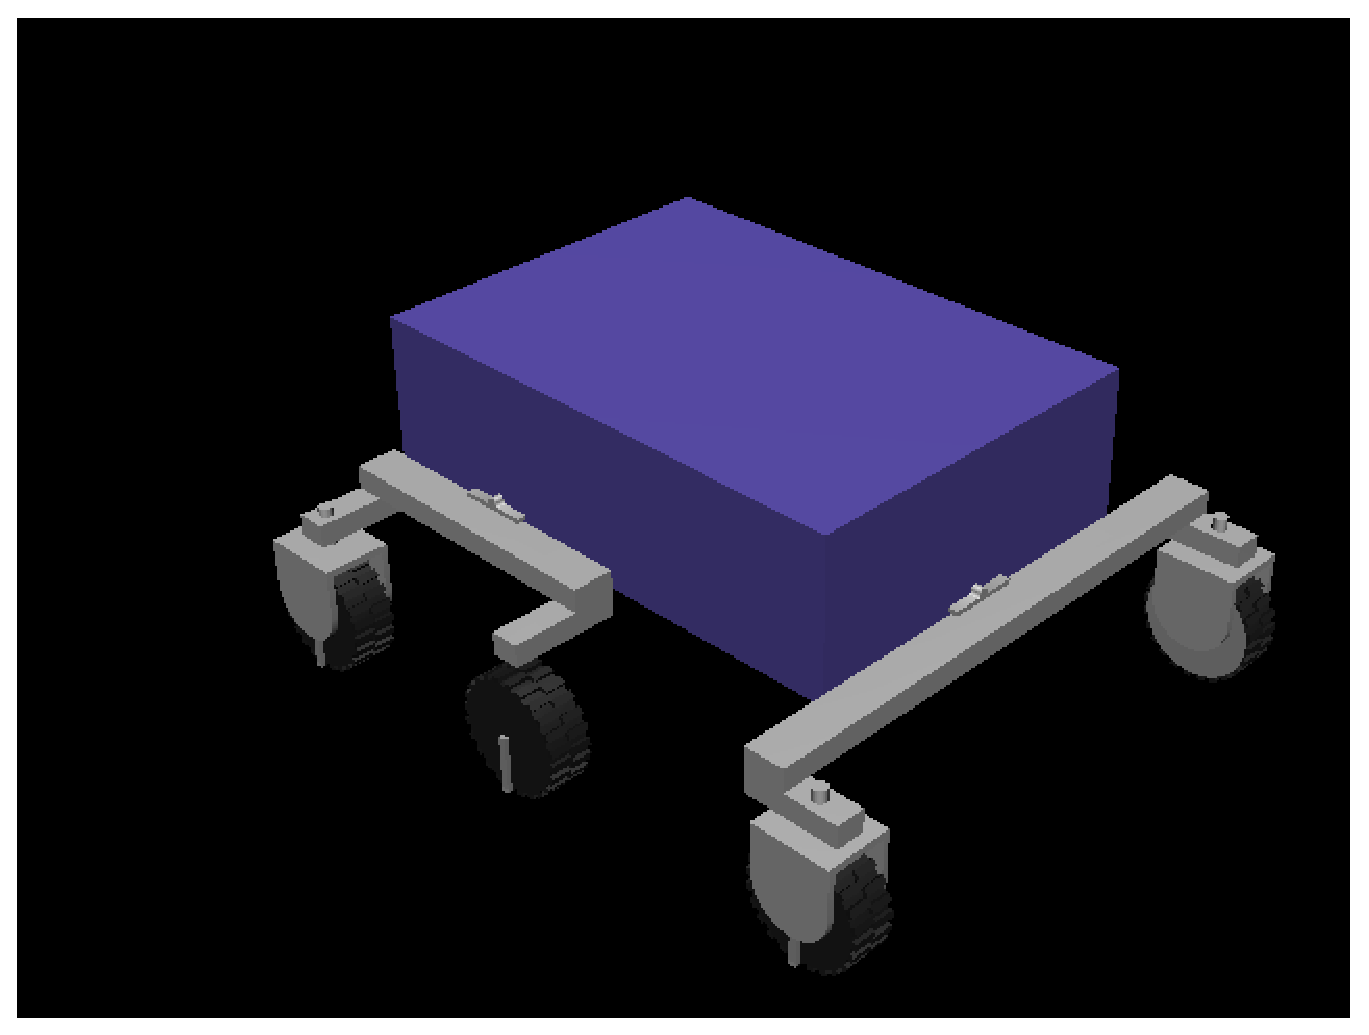
\includegraphics[width=0.8\textwidth]{rovereps}
  \caption{Assumed model of the robot}
\end{figure}

\newpage

\noindent Simplified kinematic structure of the robot is as follows:

\begin{figure}[h!]
  \centering
    \input{kkk.pdftex_t}  
  \caption{Geometry of the model}
\end{figure}

\newpage
\section{Test 1}
\label{Sec:test_1}

This test is divided into two sub-cases.

\subsection{Normal restitution coefficient set to $\boldsymbol{eps_{n} = 0.0}$}

In the first test setting rover falls freely from the height of 2 meters onto a horizontal plane.
No torques are applied in any of the joints. The only external forces acting on the rover are
the gravity and the ground reaction forces. Initial position of the rover has been set to (x, y, z) = (5, 5, 2) [m].
Friction coefficient has been set to 0.7. In this sub-case restitution coefficients (tangential and normal) have been set to zero. 

\begin{figure}[H]
  \centering
    \includegraphics[width=0.8\textwidth]{run_1}
  \caption{First test setting (arrows depict contact forces)}
\end{figure}

\noindent The following essential quantities have been plotted in this case:

\begin{figure}[H]
  \centering
    \includegraphics[width=0.8\textwidth]{xvpCOM}
  \caption{Position, velocity and reaction forces of the center of mass}
\end{figure}

\noindent \textbf{\textit{\Large{Comments}}}\\[1mm]
\noindent As seen in the figure 4, coordinate z of the center of mass of the rover decreases parabolically until the system is stable on the plane. This represents the
free-fall phase under gravity. After reaching the plane there is no rebound as the coefficient of restitution in the nonsmooth contact law has been set to zero. Impact corresponds to a 
sharp peak in the force as seen in the third sub-figure.

\noindent Also, the following complimentary quantities have been plotted:

\begin{figure}[H]
  \centering
    \includegraphics[width=0.8\textwidth]{lambdaNTS}
  \caption{Normal and tangential components of the local contact force (impulsion $\lambda$) for each wheel during impact}
\end{figure}

\begin{figure}[H]
  \centering
    \includegraphics[width=0.8\textwidth]{yNyNdot}
  \caption{$y_{N}$ - gap function (distance between contact point and the constraint function) for each wheel and $\dot{y}_{N}$ - normal component of the local contact velocity for each wheel}
\end{figure}

\noindent \textbf{\textit{\Large{Comments}}}\\[1mm]
\noindent Plots in the figure 5 correspond to forces (normal and tangential impulsions) computed in the local contact frame.
Contact forces are always computed in the local frame and then expressed in the coordinates of the system using jacobian matrix of the constraint function. 
Constraint function (gap function) used to detect the contact and the relative velocity are plotted in the figures 6. Gap function is a relative distance between two contacting
bodies and it imposes geometric constraints on the system. Once slightly below zero it will trigger a nonsmooth interaction between those bodies.\\ 

\subsection{Normal restitution coefficient set to $\boldsymbol{eps_{n} = 0.2}$}

\begin{figure}[H]
  \centering
    \includegraphics[width=0.8\textwidth]{xvpCOMrest}
  \caption{Position, velocity and reaction forces of the center of mass}
\end{figure}

\noindent \textbf{\textit{\Large{Comments}}}\\[1mm]
\noindent As the restitution coefficient has been set to a non-zero value in this case one observes multiple impacts. Impacts corresponds to peaks of forces in the third sub-figure and 
nonsmooth changes of velocity in the second sub-figure. As the energy is dissipated the magnitudes of impacts reduce in time.\\

\noindent Also, the following complimentary quantities have been plotted:

\begin{figure}[H]
  \centering
    \includegraphics[width=0.8\textwidth]{lambdaNTSrest}
  \caption{Normal and tangential components of the local contact force (impulsion $\lambda$) for each wheel during impact}
\end{figure}

\begin{figure}[H]
  \centering
    \includegraphics[width=0.8\textwidth]{yNyNdotrest}
  \caption{$y_{N}$ - gap function (distance between contact point and the constraint function) for each wheel and $\dot{y}_{N}$ - normal component of the local contact velocity for each wheel}
\end{figure}

\noindent \textbf{\textit{\Large{Comments}}}\\[1mm]
\noindent In the figure 9 one can see the gap function and relative velocity plots. With respect to the previous sub-case rebounds off the ground are visible.\\ 



\newpage
\section{Test 2}
\label{Sec:test_2}

In the second test setting rover stands still on the horizontal plane during first 50 seconds of the simulation.
However, after 50 seconds from the beginning of the simulation a constant torque $\tau = 2N$ is applied in one of the steering axes (steering axis FL)
causing its rotational motion with linear velocity. Wheel makes two full rotations around its vertical steering axis (FL). 
Other external forces acting on the rover are the gravity and ground reaction. Initial position of the center of mass of the robot
has been set to (x, y, z) = (10, 0.55, 10). 

\begin{figure}[H]
  \centering
    \includegraphics[width=0.8\textwidth]{run_2}
  \caption{Second test scenario}
\end{figure}

\noindent In this case, following quantities have been plotted:

\begin{itemize}
  \item $v_{FL}$ - angular velocity of the FL axis
\end{itemize}

\begin{figure}[H]
  \centering
    \includegraphics[width=0.8\textwidth]{vFL}
  \caption{$v_{FL}$}
\end{figure}

\begin{itemize}
  \item $x_{FL}$ - $q$ coordinate corresponding to the FL axis
\end{itemize}

\begin{figure}[H]
  \centering
    \includegraphics[width=0.8\textwidth]{xFL}
  \caption{$x_{FL}$}
\end{figure}

\begin{itemize}
  \item $\lambda_{N}$ - normal component of the contact force (impulsion) for each wheel
\end{itemize}

\begin{figure}[H]
  \centering
    \includegraphics[width=0.8\textwidth]{lambdaN2}
  \caption{$\lambda_{N}$}
\end{figure}

\begin{figure}[H]
  \centering
    \includegraphics[width=0.8\textwidth]{lambdaN2steady}
  \caption{$\lambda_{N}$ zoom view}
\end{figure}

\begin{itemize}
  \item $\lambda_{T_x}$ - tangential component of the contact force in the x direction for each wheel
\end{itemize}

\begin{figure}[H]
  \centering
    \includegraphics[width=0.8\textwidth]{lambdaTx2}
  \caption{$\lambda_{T_x}$}
\end{figure}

\begin{itemize}
  \item $\lambda_{T_z}$ - tangential component of the contact force in the z direction for each wheel
\end{itemize}

\begin{figure}[H]
  \centering
    \includegraphics[width=0.8\textwidth]{lambdaTz2}
  \caption{$\lambda_{T_z}$}
\end{figure}

\begin{itemize}
  \item $y_{N}$ - gap function (distance between contact point and the constraint function) for each wheel
\end{itemize}

\begin{figure}[H]
  \centering
    \includegraphics[width=0.8\textwidth]{yN2}
  \caption{$y_{N}$}
\end{figure}

\begin{itemize}
  \item $\dot{y}_{N}$ - normal component of the local contact velocity for each wheel
\end{itemize}

\begin{figure}[H]
  \centering
    \includegraphics[width=0.8\textwidth]{yNdot2}
  \caption{$\dot{y}_{N}$}
\end{figure}

\begin{itemize}
  \item $\dot{y}_{T_x}$ - tangential component x of the local contact velocity for each wheel
\end{itemize}

\begin{figure}[H]
  \centering
    \includegraphics[width=0.8\textwidth]{yTxdots2}
  \caption{$\dot{y}_{T_x}$}
\end{figure}

\begin{itemize}
  \item $\dot{y}_{T_z}$ - tangential component z of the local contact velocity for each wheel
\end{itemize}

\begin{figure}[H]
  \centering
    \includegraphics[width=0.8\textwidth]{yTzdots2}
  \caption{$\dot{y}_{T_z}$}
\end{figure}


\newpage
\section{Test 3}
\label{Sec:test_3}

In the third test setting rover's parcour is divided into six time intervals with different values of torques applied to the wheels:

\begin{enumerate} 
  \item $0s < t_s < 50s$, $\tau = 0N$           
  \item $50s < t_s < 100s$, $\tau = 700N$        
  \item $100s < t_s < 150s$, $\tau = 0N$         
  \item $150s < t_s < 220s$, $\tau = -500N$
  \item $220s < t_s < 300s$, $\tau = 0N$         
  \item $300s < t_s < 400s$, $\tau = -500N$ 
\end{enumerate}

\noindent Other external forces acting on the rover are the gravity and ground reaction. Initial position of the center of mass of the robot
has been set to (x, y, z) = (18, 0.55, 10). In the $5^{th}$ phase rover effectively stops its motion until negative torques are applied.

\begin{figure}[H]
  \centering
    \includegraphics[width=0.8\textwidth]{run_1}
  \caption{Third test scenario}
\end{figure}

\noindent In this case, following quantities have been plotted:

\begin{itemize}
  \item $x_{COM}$ - mass center coordinates
\end{itemize}

\begin{figure}[H]
  \centering
    \includegraphics[width=0.8\textwidth]{xCOM3}
  \caption{$x_{COM}$}
\end{figure}

\begin{itemize}
  \item $x_{wheels}$ - wheels angular displacement 
\end{itemize}

\begin{figure}[H]
  \centering
    \includegraphics[width=0.8\textwidth]{xWHEELS3}
  \caption{$x_{wheels}$}
\end{figure}

\begin{itemize}
  \item $v_{COM}$ - mass center velocity
\end{itemize}

\begin{figure}[H]
  \centering
    \includegraphics[width=0.8\textwidth]{vCOM3}
  \caption{$v_{COM}$}
\end{figure}

\begin{itemize}
  \item $v_{wheels}$ - wheels angular velocity
\end{itemize}

\begin{figure}[H]
  \centering
    \includegraphics[width=0.8\textwidth]{vWHEELS3}
  \caption{$v_{wheels}$}
\end{figure}

\begin{itemize}
  \item $R_{COM}$ - reaction forces of center of mass in lagrangian coordinates
\end{itemize}

\begin{figure}[H]
  \centering
    \includegraphics[width=0.8\textwidth]{pCOM3}
  \caption{$R_{COM}$}
\end{figure}

\begin{itemize}
  \item $R_{wheels}$ - reaction forces of wheels in lagrangian coordinates
\end{itemize}

\begin{figure}[H]
  \centering
    \includegraphics[width=0.8\textwidth]{pWHEELS3}
  \caption{$R_{wheels}$}
\end{figure}

\begin{itemize}
  \item $\lambda_{N}$ - normal component of the contact force (impulsion) for each wheel
\end{itemize}

\begin{figure}[H]
  \centering
    \includegraphics[width=0.8\textwidth]{lambdaN3}
  \caption{$\lambda_N$}
\end{figure}

\begin{itemize}
  \item $\lambda_{T_x}$ - tangential component of the contact force in the x direction for each wheel
\end{itemize}

\begin{figure}[H]
  \centering
    \includegraphics[width=0.8\textwidth]{lambdaTx3}
  \caption{$\lambda_{T_x}$}
\end{figure}

\begin{itemize}
  \item $\lambda_{T_z}$ - tangential component of the contact force in the z direction for each wheel
\end{itemize}

\begin{figure}[H]
  \centering
    \includegraphics[width=0.8\textwidth]{lambdaTz3}
  \caption{$\lambda_{T_z}$}
\end{figure}

\begin{itemize}
  \item $y_{N}$ - gap function (distance between contact point and the constraint function) for each wheel
\end{itemize}

\begin{figure}[H]
  \centering
    \includegraphics[width=0.8\textwidth]{yN3}
  \caption{$y_N$}
\end{figure}

\begin{itemize}
  \item $\dot{y}_{N}$ - normal component of the local contact velocity for each wheel
\end{itemize}

\begin{figure}[H]
  \centering
    \includegraphics[width=0.8\textwidth]{yNdot3}
  \caption{$\dot{y}_{N}$}
\end{figure}

\begin{itemize}
  \item $\dot{y}_{T_x}$ - tangential component x of the local contact velocity for each wheel
\end{itemize}

\begin{figure}[H]
  \centering
    \includegraphics[width=0.8\textwidth]{yTxdots3}
  \caption{$\dot{y}_{T_x}$}
\end{figure}

\begin{itemize}
  \item $\dot{y}_{T_z}$ - tangential component z of the local contact velocity for each wheel
\end{itemize}

\begin{figure}[H]
  \centering
    \includegraphics[width=0.8\textwidth]{yTzdots3}
  \caption{$\dot{y}_{T_z}$}
\end{figure}


\newpage
\section{Test 4}
\label{Sec:test_4}

In the fourth test setting rover is set to stand steadily on an inclined plane.
Inclination angle of the slope has been set to 10$^\circ$. Torques applied to the wheels counterbalance torques caused by
the gravity. After initial period higher torques are applied to the wheels which cause the robot to drive upwards. Blocking torques are equal to  
$\tau_{b} = -0.87072Nm$. During the second phase of motion linearly varying torques are applied to all wheels. 

\begin{figure}[H]
  \centering
    \includegraphics[width=0.8\textwidth]{run_4}
  \caption{Fourth test scenario}
\end{figure}

\noindent Rover's parcour has been devided into two phases:

\begin{enumerate} 
  \item $0s < t_s < 30s$, $\tau_{b}$ $-$  $constant$ $blocking$ $torques$           
  \item $30s < t_s < 40s$, $\tau_{m}$ $-$ $linearly$ $increasing$ $torques$        
\end{enumerate}

\noindent Friction coefficient has been set to 0.8. Restitution coefficients (tangential and normal) have been set to zero.\\[1mm] 
\noindent In this case, following essential quantities have been plotted:

\begin{figure}[H]
  \centering
    \includegraphics[width=0.8\textwidth]{xvpCOM4}
  \caption{$x_{COM}$ - mass center coordinates}
\end{figure}

\noindent \textbf{\textit{\Large{Comments}}}\\[1mm]
\noindent Two phases are distinguished in this case. In the figure 19 one can see that in the first phase rover is motionless because of the constant blocking torques applied to all wheels.
These torques through friction nullify the effect of gravity on the system. Coordinates of the center of mass are constant until the second phase. This means that the friction-contact model is efficient in the sense
that it matches closely physical behavior of the phenomenon. One can see this more clearly in the velocity curve where the velocity of the center of mass is zero in the first phase of motion.
Nonsmooth friction-contact model allows for this effect as it does not rely on regularization of friction laws. Last curve in the figure 19 represents the ground reaction forces applied to the mass center of the system. 
This force increases very slightly as the rover starts moving upwards because of the friction force.\\

\noindent Following additional quantities have been plotted:

\begin{figure}[H]
  \centering
    \includegraphics[width=0.8\textwidth]{lambdaNTS4}
  \caption{$\lambda_{N}$, $\lambda_{T_x}$, $\lambda_{T_z}$ - normal and tangential components of the contact force (impulsion) for each wheel}
\end{figure}

\begin{figure}[H]
  \centering
    \includegraphics[width=0.8\textwidth]{yTxdotyTzdot4}
  \caption{$\dot{y}_{T_x}$, $\dot{y}_{T_y}$ - tangential components of the local relative velocity for each wheel}
\end{figure}

\noindent \textbf{\textit{\Large{Comments}}}\\[1mm]
\noindent In the figure 20 one can see normal and tangential components of the local contact forces. Immediate observation is that the projections of forces oscillate during the first phase of motion. This
is due to the fact that contact solver finds a different solution to the friction-contact problem at each time instant.\\


\newpage
\section{Test 5}
\label{Sec:test_5}

In the fifth test setting the rover is posed on and inclined plane.
Inclination angle of the slope has been set to 10$^\circ$. After the 10$^{th}$ second of simulation a simple PD controller
is set using position and velocity of the center of mass, in order to stop the rover on the slope. Rover stops effectively at $t = 25s$. 
Friction coefficient has been set to 0.8. Restitution coefficients (tangential and normal) have been set to zero. 

\begin{figure}[H]
  \centering
    \includegraphics[width=0.8\textwidth]{run_5}
  \caption{Fifth test scenario}
\end{figure}

\noindent In this setting we are mostly interested in two phases:

\begin{enumerate} 
  \item $0s < t_s < 10s$
  \item $10s < t_s < 40s$
\end{enumerate}

\noindent In this case, following essential quantities have been plotted:

\begin{figure}[H]
  \centering
    \includegraphics[width=0.8\textwidth]{xvpCOM5}
  \caption{position, velocity and reaction force of the mass center}
\end{figure}

\noindent \textbf{\textit{\Large{Comments}}}\\[1mm]
\noindent One can clearly see two phases of motion of the rover. In the end of the second phase rover stops its motion on the inclined plane which once again
demonstrates the efficiency of the nonsmooth friction-contact law. This can be seen in the figure 23 where in the second phase velocity components converge towards zero. 
This effect corresponding to a true nature of friction and can be captured in numerical experiments using nonsmooth laws. Using regularized laws to describe friction would not allow the system to retain non-zero torques with zero velocity.\\

\noindent Following additional quantities have been plotted:

\begin{figure}[H]
  \centering
    \includegraphics[width=0.8\textwidth]{lambdaNTS5}
  \caption{$\lambda_{N}$ - normal component of the contact force (impulsion) for each wheel}
\end{figure}

\begin{figure}[H]
  \centering
    \includegraphics[width=0.8\textwidth]{yTxdotyTzdot5}
  \caption{$\dot{y}_{T_z}$ - tangential component z of the local contact velocity for each wheel}
\end{figure}

\noindent \textbf{\textit{\Large{Comments}}}\\[1mm]
\noindent As in the previous test setting, an immediate observation comes into mind as to the oscillations in the figure 24. Indeed, it is the same reason as previously that they appear in the plot.\\



\newpage
\section{Test 6}
\label{Sec:test_6}

In the sixth test setting rover is dropped onto the horizontal plane from the height of $2$ $m$. After $10$ $s$ linearly varying torques are applied to all wheels. 
A spherical obstacle has been set in front of the rover. The obstacle is in the form of a sphere which protudes outside the plane.
Center of the sphere has been set so that the protrusion is equal to $20$ $cm$. Coefficient of friction has been set to 0.3 whereas the coefficient of restitution to 0.

\begin{figure}[H]
  \centering
    \includegraphics[width=0.8\textwidth]{run_6}
  \caption{Sixth test scenario}
\end{figure}

\noindent In this case, the following essential quantities have been plotted:

\begin{figure}[H]
  \centering
    \includegraphics[width=0.8\textwidth]{xvpCOM6}
  \caption{position, velocity and reaction forces of the mass center of the rover}
\end{figure}

\noindent \textbf{\textit{\Large{Comments}}}\\[1mm]
\noindent In this setting attention can be drawn to the spherical obstacle crossing. In the figure 27 in the first sub-plot on can see $z$ coordinate evolution of the mass center of the robot. 
It is clearly seen how around 11$^{th}$ minute rover mounts the sphere. In the sub-plot below one can see the evolution of velocities of the mass center where several small jumps occur in the 
$y$ and $z$ dimension as a result of impacts. Velocity in the $x$ direction is clearly larger as the rover moves along the $x$ axis. Impacts are more clearly seen in the third sub-plot with each peak 
corresponding to an impact.\\
 
\noindent Following additional quantities have also been plotted:

\begin{figure}[H]
  \centering
    \includegraphics[width=0.8\textwidth]{lambdaNTS6}
  \caption{$\lambda_{N}$, $\lambda_{T_x}$, $\lambda_{T_y}$ - normal component of the contact force (impulsion) for each wheel (interaction with the plane)}
\end{figure}

\begin{figure}[H]
  \centering
    \includegraphics[width=0.8\textwidth]{lambdaNTS6sphere}
  \caption{$\lambda_{N}$, $\lambda_{T_x}$, $\lambda_{T_y}$ - normal component of the contact force (impulsion) for each wheel (interaction with the sphere)}
\end{figure}

\noindent \textbf{\textit{\Large{Comments}}}\\[1mm]
\noindent In the figure 28 and 29 local contact forces have been plotted seen from the interaction with plane and sphere respectively. One can observe several peaks corresponding to the
phase of the simulation when the obstacle is being crossed.\\


\newpage
\section{Test 7}
\label{Sec:test_7}

In the seveth test setting rover is dropped onto the horizontal plane.
An obstacle in the form of a horizontal step of height $0.1$ $m$ has been set in front of the rover.
At certain point rover starts moving towards the step and crosses it mounting on the higher plane.

\begin{figure}[H]
  \centering
    \includegraphics[width=0.8\textwidth]{run_7}
  \caption{Seventh test scenario}
\end{figure}

\noindent In this case, following quantities have been plotted:

\begin{itemize}
  \item $x_{COM}$ - mass center coordinates
\end{itemize}

\begin{figure}[H]
  \centering
    \includegraphics[width=0.8\textwidth]{xCOM7}
  \caption{$x_{COM}$}
\end{figure}

\begin{itemize}
  \item $x_{wheels}$ - wheels angular displacement 
\end{itemize}

\begin{figure}[H]
  \centering
    \includegraphics[width=0.8\textwidth]{xWHEELS7}
  \caption{$x_{wheels}$}
\end{figure}

\begin{itemize}
  \item $v_{COM}$ - mass center velocity
\end{itemize}

\begin{figure}[H]
  \centering
    \includegraphics[width=0.8\textwidth]{vCOM7}
  \caption{$v_{COM}$}
\end{figure}

\begin{itemize}
  \item $v_{wheels}$ - wheels angular velocity
\end{itemize}

\begin{figure}[H]
  \centering
    \includegraphics[width=0.8\textwidth]{vWHEELS7}
  \caption{$v_{wheels}$}
\end{figure}

\begin{itemize}
  \item $R_{COM}$ - reaction forces of center of mass in lagrangian coordinates
\end{itemize}

\begin{figure}[H]
  \centering
    \includegraphics[width=0.8\textwidth]{pCOM7}
  \caption{$R_{COM}$}
\end{figure}

\begin{itemize}
  \item $R_{wheels}$ - reaction forces of wheels in lagrangian coordinates
\end{itemize}

\begin{figure}[H]
  \centering
    \includegraphics[width=0.8\textwidth]{pWHEELS7}
  \caption{$R_{wheels}$}
\end{figure}


\end{document}
 
